\documentclass[conference]{IEEEtran}
\IEEEoverridecommandlockouts

\usepackage{graphicx}
\usepackage{booktabs}
\usepackage{amsmath}
\usepackage{amssymb}
\usepackage{cite}
\usepackage[hidelinks]{hyperref}
\usepackage[capitalise,nameinlink]{cleveref}
\crefname{figure}{Fig.}{Figs.}
\Crefname{figure}{Fig.}{Figs.}
\crefname{table}{Table}{Tables}
\crefname{section}{Section}{Sections}
\crefname{equation}{Eq.}{Eqs.}

\graphicspath{{../figures/}}
\renewcommand{\topfraction}{0.9}
\renewcommand{\dbltopfraction}{0.9}
\renewcommand{\textfraction}{0.1}
\renewcommand{\floatpagefraction}{0.8}
\renewcommand{\dblfloatpagefraction}{0.8}
\setcounter{topnumber}{3}
\setcounter{dbltopnumber}{3}
\raggedbottom

% Style notes: active voice, present tense, American English. Italic marks a term at its
% definition; bold marks best values in tables only. Each paragraph starts with a TL;DR comment.

\begin{document}

\title{Auditing SHAP Explanations Against Latent Failure Mechanisms in Predictive Maintenance}

\author{\IEEEauthorblockN{Koshik Debanath}
\IEEEauthorblockA{Independent Researcher\\
koshik.debanath@gmail.com}}

\maketitle

\begin{abstract}
% X: what and why
Analysts use SHAP (SHapley Additive exPlanations) to explain predictive maintenance (PdM)
classifiers, but rarely test whether an explanation matches the physical cause of failure.
% Y: why hard
Such a test needs ground truth about why each failure happened, which PdM data rarely provides, and
we show that an obvious test for it certifies a model fitted to shuffled labels.
% Z: what we do
We use the AI4I~2020 dataset, whose failure label is the logical OR of five separately recorded
failure mechanisms. We train a classifier on the combined label only and then audit its attributions
per mechanism: on the rows where a mechanism occurred, we measure the share of mean absolute SHAP
value that falls on the features the mechanism's trigger rule uses, and compare it against 100
models retrained on permuted labels.
% 1: evidence
The tuned XGBoost model (test precision 1.00, recall 0.82, F1 0.90) passes all four physical
mechanisms ($p \le 0.02$). A model trained on permuted labels fails all four, and a model given a
synthetic shortcut sensor fails only the mechanism the shortcut imitates, although its F1 of 0.86
exceeds every non-XGBoost baseline. The verdicts hold on rows with a single mechanism, and three of
four mechanisms pass with raw sensor features alone.
\end{abstract}

\begin{IEEEkeywords}
explainable AI, SHAP, predictive maintenance, faithfulness evaluation, model randomization,
class imbalance
\end{IEEEkeywords}

\section{Introduction}
\label{sec:intro}

% X: explanations of PdM models are trusted without being tested against the true cause
Predictive maintenance (PdM) systems predict equipment failure from sensor readings, and their
users often ask why a model flags a machine. The common answer is a post-hoc attribution such as
SHAP~\cite{lundberg2017shap}, presented as evidence that the model relies on sensible inputs. The
explanation itself is rarely tested against the actual cause of the failure. A classifier with high
accuracy can still rely on a correlate of failure rather than on its cause, and a plausible SHAP plot
does not reveal this~\cite{cummins2024survey}.

% Y: the test needs per-failure causes, which data rarely has; naive tests are confounded
Testing an explanation against causes requires knowing, for each failure, which mechanism produced
it. Industrial datasets seldom record this. A second difficulty is statistical: rows that belong to a
failure mechanism are, by definition, extreme in that mechanism's features. We find that a test
which ignores this effect passes a model fitted to shuffled labels (\cref{sec:controls}).

% Z: AI4I records the mechanism separately from the label the model sees
The AI4I~2020 dataset~\cite{matzka2020explainable} provides the missing ground truth. Its target,
\texttt{Machine failure}, is the logical OR of five mechanism flags: tool wear failure (TWF), heat
dissipation failure (HDF), power failure (PWF), overstrain failure (OSF), and random failure (RNF).
The first four follow published trigger rules on the sensor variables (\cref{tab:mechanisms}); RNF
does not. We train on the combined label only and keep the flags for an audit. For each mechanism, we
compute the share of the model's SHAP attribution that falls on the features its trigger rule uses,
and we compare that share against models retrained on permuted labels, following the randomization
logic of Adebayo et al.~\cite{adebayo2018sanity}.

% 1: hypotheses and how we test them
We test three hypotheses:
\begin{itemize}
  \item \textbf{H1:} for each physical mechanism, a well-performing model concentrates attribution on
    that mechanism's trigger features more than permuted-label models do;
  \item \textbf{H2:} the audit rejects models whose attributions are known to be wrong -- a model
    trained on permuted labels and a model given a synthetic shortcut sensor -- and identifies the
    affected mechanism;
  \item \textbf{H3:} a naive null, which compares random failure rows under the same model, does not
    separate these cases.
\end{itemize}
The results support all three (\cref{fig:overview}).

\begin{figure}[t]
\centering
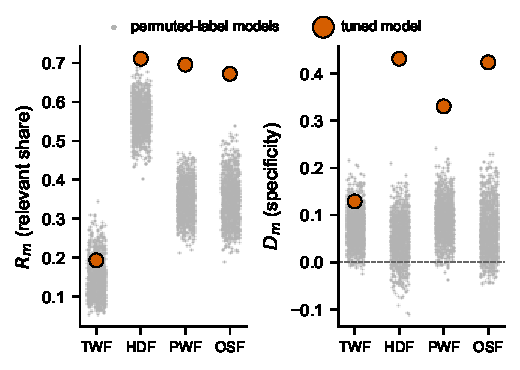
\includegraphics[width=\columnwidth]{audit_overview.pdf}
\caption{Audit statistic $R_m$ (\cref{eq:share}) for each physical mechanism. Gray points: 100
models from the tuned pipeline retrained on permuted labels. The tuned model lies above all or nearly
all of them for every mechanism. The model with a strong shortcut sensor falls below them only for
HDF, the mechanism the shortcut imitates (its own null gives the same verdict; \cref{tab:controls}).}
\label{fig:overview}
\end{figure}

% 2: contributions, separated from prior work
Our contributions are:
\begin{itemize}
  \item a per-mechanism audit of SHAP attributions that uses mechanism labels already present in a
    public PdM benchmark, with a model-randomization null (\cref{sec:method});
  \item evidence that a naive within-model null is confounded: it passes a model trained on permuted
    labels (\cref{sec:controls});
  \item positive controls showing that the audit fails when it should and localizes the failure to
    one mechanism, plus a single-mechanism analysis and a raw-feature ablation
    (\cref{sec:controls});
  \item an imbalance-aware benchmark of seven model families on AI4I~2020 with confidence intervals,
    and code that reproduces every number in this paper.
\end{itemize}
The resampling methods, models, and explainer are existing tools; the audit design, the null
analysis, and the controls are ours.

\section{Related Work}
\label{sec:related}

% XAI on AI4I: global reporting, no mechanism-level test; we compare predictive results instead
\textit{Explanations on AI4I~2020.} Matzka~\cite{matzka2020explainable} introduced the dataset with
local explanations for individual predictions. Zhao et al.~\cite{milling2025shap} report global SHAP
importance for tree ensembles on it. Neither work tests attributions against the mechanism flags,
and neither defines a pass/fail criterion, so there is no audit to compare against. We compare
predictive performance instead: Tseng~\cite{physicsinformed2026} reports random forest
positive-class F1 of 0.722 with engineered features, and Khemani and
Qureshi~\cite{connectedvehicles2026} report LightGBM macro-F1 of $0.814 \pm 0.012$ under 5-fold
cross-validation with resampling inside the folds (\cref{tab:prior}).

% Faithfulness with synthetic ground truth: measures fidelity to the model, not the mechanism
\textit{Faithfulness evaluation.} Liu et al.~\cite{liu2021synthetic} generate synthetic data with
known conditional distributions, which makes ground-truth Shapley values computable. Such benchmarks
measure whether an explainer reports the model's behavior faithfully. Our question differs: given a
faithful explainer, does the model's behavior match the process that generated the failures? Their
metrics need closed-form access to the data distribution, which AI4I~2020 does not provide for its
recorded mechanisms, so we do not use them as baselines.

% Randomization tests: we adopt the logic, but apply it to a different question
\textit{Randomization tests.} Adebayo et al.~\cite{adebayo2018sanity} show that some saliency
methods give nearly the same explanation for a trained model and a randomized one, and propose
randomization as a sanity check on explainers. We adopt the same logic but apply it to the model:
permuted-label models define what attribution looks like when the model has no relation to the
failure mechanisms.

% Causal PdM: different goal
\textit{Causal PdM.} Dhande et al.~\cite{causalbenchmark2026} fit causal structural models on a CNC
failure dataset of similar size to optimize maintenance cost. They replace the correlational model;
we keep it and test its explanation, so the two approaches address different questions.

\section{Background and Problem Setting}
\label{sec:background}

% SHAP basics needed to read the statistic
\textit{SHAP.} For a model $f$ and input $x$ with $d$ features, SHAP assigns each feature $j$ an
attribution $\phi_j(x)$, its Shapley value with respect to the model output, such that
$f(x) = \phi_0 + \sum_{j=1}^{d} \phi_j(x)$, where $\phi_0$ is the expected
output~\cite{lundberg2017shap}. For tree ensembles, TreeSHAP computes these values exactly in
polynomial time. We use $|\phi_j(x)|$ as the magnitude of feature $j$'s contribution to the
prediction for $x$.

% Problem setting and notation
\textit{Problem setting.} We observe rows $(x_i, y_i, z_i)$, where $x_i$ is the sensor vector,
$y_i \in \{0, 1\}$ is the failure label, and $z_i \in \{0, 1\}^M$ holds $M$ mechanism flags. We train
$f$ on $(x_i, y_i)$ only; the flags $z$ never enter training. For each mechanism $m$, domain rules
specify a set $E_m$ of features the mechanism's trigger depends on. The audit asks whether, on the
rows $S_m = \{i : z_{i,m} = 1\}$, the attributions of $f$ concentrate on $E_m$. Two assumptions are
unusual: $E_m$ must be known from domain knowledge, and the flags must exist for at least some
failures, even if the deployed model never sees them.

\section{Audit Method}
\label{sec:method}

% Statistic definition
For mechanism $m$ and feature $j$, the mean attribution magnitude on the mechanism's rows is
\begin{equation}
  I_{m,j} = \frac{1}{|S_m|} \sum_{i \in S_m} \left| \phi_j(x_i) \right|.
\end{equation}
The \textit{relevant share} is the fraction of that attribution which falls on the trigger features,
\begin{equation}
  R_m = \sum_{j \in E_m} I_{m,j} \Big/ \sum_{j=1}^{d} I_{m,j}.
  \label{eq:share}
\end{equation}
$R_m$ lies in $[0, 1]$; a value near 1 means that, on the mechanism's rows, almost all attribution
falls on the trigger features.

% Naive null and its confound
\textit{Naive null.} An obvious test compares $R_m$ with the same statistic computed on random,
equally sized subsets of all failure rows under the same model. This null passes a model fitted to
shuffled labels on every mechanism (\cref{sec:controls}), so it does not measure what the model
uses. A likely reason is that rows in $S_m$ are extreme in the features of $E_m$, because the trigger
rule selects them by those features, and that $|\phi_j|$ tends to be larger at atypical values of
$x_j$ whatever the model has fitted.

% Model-randomization null
\textit{Model-randomization null.} We instead retrain the full pipeline -- same features,
resampling, and hyperparameters -- $K$ times on permuted training labels and compute $R_m$ for each
retrained model. These models see the same rows but have no relation to the mechanisms. A mechanism
passes if
\begin{equation}
  p_m = \frac{1 + \#\{k : R^{(k)}_m \ge R_m\}}{K + 1} < 0.05,
\end{equation}
where $R^{(k)}_m$ is the statistic of the $k$-th permuted model. The smallest attainable $p$ is
$1/(K+1)$.

% RNF
\textit{Random failures.} RNF has no trigger features. Its statistic is the share of the single
largest feature, $\max_j I_{m,j} / \sum_j I_{m,j}$, and RNF passes if the model is not more
concentrated than the permuted models ($p \ge 0.05$).

% Controls validate the audit itself
\textit{Controls.} An audit is informative only if it fails on models that should fail. We therefore
run it on two models with known-wrong attributions (\cref{sec:setup}) and require that it rejects
them.

\section{Experimental Setup}
\label{sec:setup}

% Dataset
\textit{Dataset.} AI4I~2020 has 10{,}000 rows: a quality variant \texttt{Type} $\in \{L, M, H\}$
(50/30/20\%), five process variables (air and process temperature, rotational speed, torque, tool
wear), the failure label, and the five mechanism flags. 339 rows (3.39\%) are failures.

% Label inconsistencies and their consequence
The released labels depart from the stated OR rule. 24 rows carry more than one mechanism flag,
9 failures carry none, and 18 of the 19 RNF rows have \texttt{Machine failure}~$= 0$. Because the
RNF rows are almost all non-failures, the RNF check is weak; the positive controls provide the
evidence that the audit discriminates. We run the audit on all flagged rows and, separately, on
rows with exactly one mechanism flag.

\begin{table}[t]
\centering
\caption{Failure mechanisms in AI4I~2020~\cite{matzka2020explainable} and their trigger features
$E_m$; counts as released. The TWF failure point is random within the window.}
\label{tab:mechanisms}
\footnotesize
\setlength{\tabcolsep}{3pt}
\begin{tabular}{@{}lp{3.4cm}p{2.9cm}r@{}}
\toprule
Mech. & Trigger & $E_m$ & $n$ \\
\midrule
TWF & tool wear at a random point in 200--240\,min & tool wear & 46 \\
HDF & (process $-$ air temp.) $< 8.6$\,K and speed $< 1380$\,rpm & both temps., their difference,
  speed & 115 \\
PWF & torque $\times$ speed (rad/s) outside [3500, 9000]\,W & torque, speed, power & 95 \\
OSF & tool wear $\times$ torque above 11/12/13k\,min$\cdot$Nm (L/M/H) & tool wear, torque,
  overstrain, its ratio & 98 \\
RNF & 0.1\% chance, independent of the process & -- & 19 \\
\bottomrule
\end{tabular}
\end{table}

% Features and leakage
\textit{Features.} We derive four features from the trigger rules without using the flags:
\textit{power} (torque $\times$ speed), \textit{temperature difference} (process $-$ air),
\textit{overstrain} (tool wear $\times$ torque), and \textit{overstrain ratio} (overstrain divided by
the type-specific limit). We drop the identifiers. The mechanism flags are components of the label,
so we exclude them from the features and keep them for the audit only.

% Split, resampling, models
\textit{Training.} We split the data 70/20/10 into training, validation, and test sets, stratified by
label, and fit scaling and one-hot encoding on the training set only. We compare three oversamplers
-- the synthetic minority over-sampling technique (SMOTE)~\cite{chawla2002smote},
Borderline-SMOTE~\cite{han2005borderline}, and adaptive synthetic sampling
(ADASYN)~\cite{he2008adasyn} -- by the validation F1 of a default XGBoost~\cite{chen2016xgboost}
model, and use the best one, Borderline-SMOTE, for all models. We train seven model families on the
resampled training set (\cref{tab:config}) and evaluate them on the untouched validation and test
sets.

\begin{table}[t]
\centering
\caption{Model settings. Unlisted hyperparameters are library defaults (scikit-learn 1.9.1,
XGBoost 3.4.1, PyTorch 2.14.0); random seed 42.}
\label{tab:config}
\footnotesize
\begin{tabular}{@{}lp{5.6cm}@{}}
\toprule
Model & Settings \\
\midrule
Logistic regression & max.\ 1000 iterations \\
SVM & radial basis function (RBF) kernel, probability outputs \\
$k$-NN & $k = 7$ \\
Decision tree & max.\ depth 10 \\
Random forest & 300 trees, max.\ depth 12 \\
XGBoost & 300 trees, max.\ depth 6, learning rate 0.1 \\
XGBoost (tuned) & 200 trees, max.\ depth 8, learning rate 0.2, subsample 0.8, column sample 1.0,
  min.\ child weight 1, $\gamma = 0$ \\
MLP (PyTorch) & 64 and 32 hidden units, ReLU, batch norm, dropout 0.3/0.2; Adam (learning rate
  $10^{-3}$, weight decay $10^{-5}$), binary cross-entropy, batch 64, 40 epochs \\
\bottomrule
\end{tabular}
\end{table}

% Selection, tuning, uncertainty
\textit{Selection and tuning.} We select models on the validation set only. XGBoost has the highest
validation F1 (0.826, against 0.739 for random forest), so we tune it with a 40-iteration randomized
search under 5-fold stratified cross-validation, scored on F1, over depth 3--8, 200--600 trees,
learning rate 0.01--0.2, subsample and column sample 0.6--1.0, minimum child weight 1--5, and
$\gamma$ 0--0.3. We set the decision threshold to maximize F1 on the validation precision-recall (PR)
curve. We report exact binomial (Clopper--Pearson) 95\% confidence intervals (CIs) for precision and
recall and a 5{,}000-sample stratified bootstrap for F1 and the area under the receiver operating
characteristic curve (ROC-AUC). We also run 5-fold stratified cross-validation with every step refit
inside each fold.

% Audit implementation
\textit{Audit.} We compute TreeSHAP values of the tuned model on all flagged rows, because the test
set alone contains too few TWF and RNF rows; the audit uses no labels for training. We use $K = 100$
permuted-label models, so the smallest attainable $p$ is 0.0099.

% Control variants
\textit{Controls.} We audit five variants, each with its own 100-model null: (i) the tuned model on
single-mechanism rows only; (ii) the same pipeline without the four derived features (\textit{raw
features}), to test whether the derived features make the audit circular; (iii) a model trained on
permuted labels, which should fail every mechanism; (iv--v) models given an extra synthetic
``sensor'' with no physical role that tracks HDF, at two noise levels. The \textit{weak shortcut} is
$\mathcal{N}(0,1) + 1.5\,z_{\mathrm{HDF}}$ and the \textit{strong shortcut} is
$\mathcal{N}(0,0.1) + z_{\mathrm{HDF}}$. The shortcut sensor is not in $E_{\mathrm{HDF}}$, so a model
that relies on it should fail the HDF audit.

\section{Results and Discussion}
\label{sec:results}

\begin{figure*}[t]
\centering
\begin{minipage}[b]{0.49\textwidth}
\centering
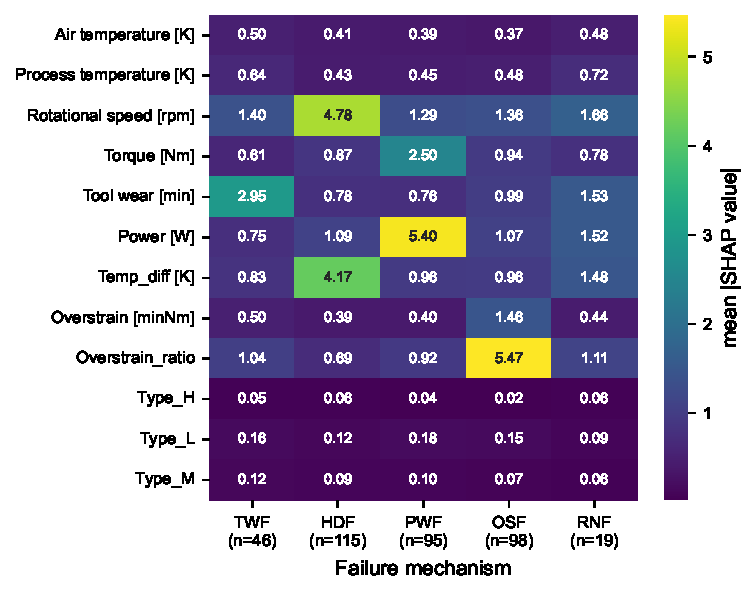
\includegraphics[width=0.95\linewidth]{shap_crosscheck_heatmap.pdf}\\
\small (a) Mean $|\phi_j|$ on the rows of each mechanism
\end{minipage}\hfill
\begin{minipage}[b]{0.47\textwidth}
\centering
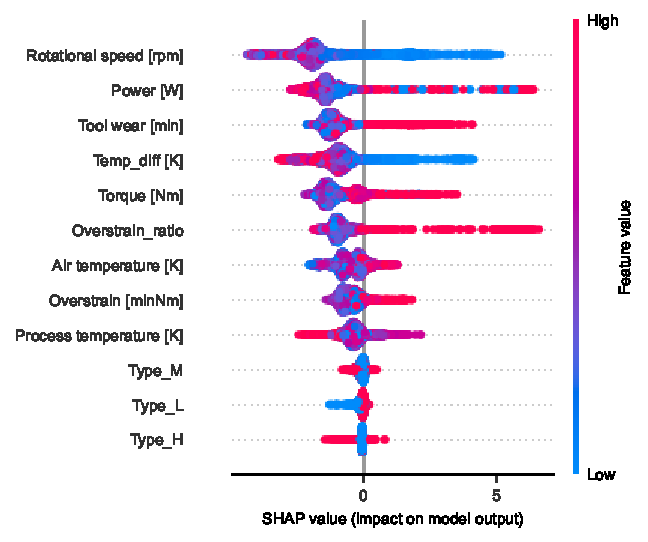
\includegraphics[width=0.95\linewidth]{shap_summary.pdf}\\
\small (b) Global SHAP summary on all rows
\end{minipage}
\caption{SHAP attributions of the tuned model. The audit tests the per-mechanism view (a); the global
view (b) ranks features overall but does not separate the mechanisms.}
\label{fig:shap}
\end{figure*}

\begin{figure*}[t]
\centering
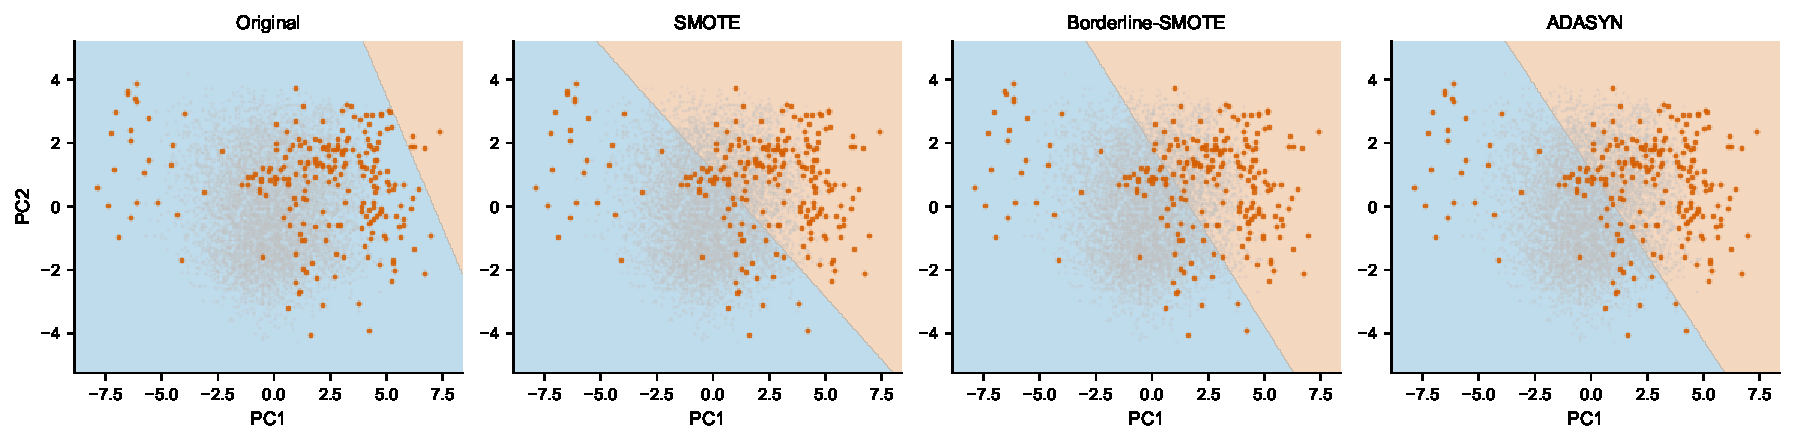
\includegraphics[width=0.9\textwidth]{decision_boundary_2d.pdf}
\caption{Logistic regression decision boundary on a two-dimensional principal component analysis
(PCA) projection of the training data, for each resampler.}
\label{fig:boundary}
\end{figure*}

\begin{figure*}[t]
\centering
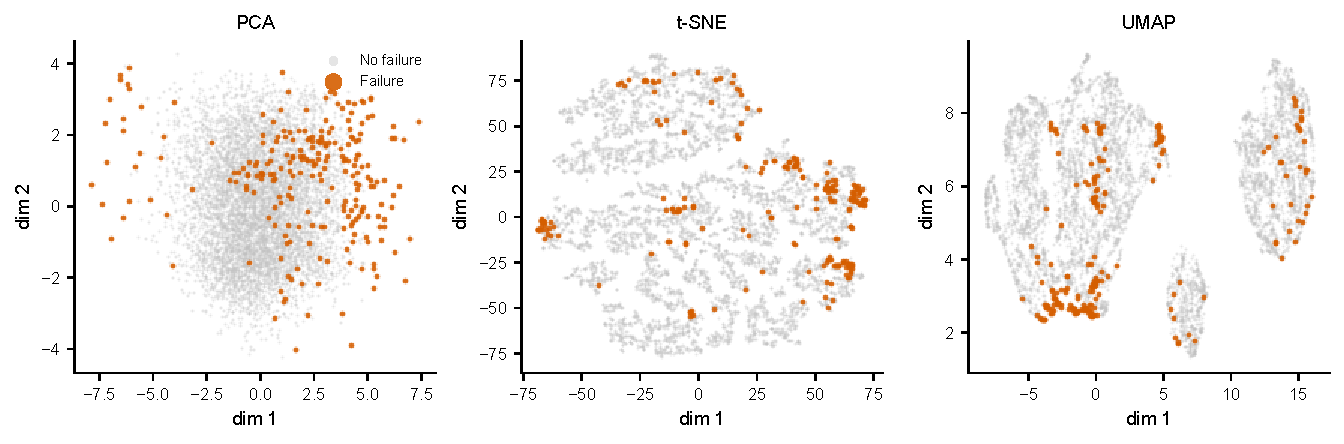
\includegraphics[width=0.8\textwidth]{dimred_comparison.pdf}
\caption{PCA, t-SNE, and UMAP projections of the training data, colored by \texttt{Machine failure}.}
\label{fig:dimred}
\end{figure*}

\begin{figure*}[t]
\centering
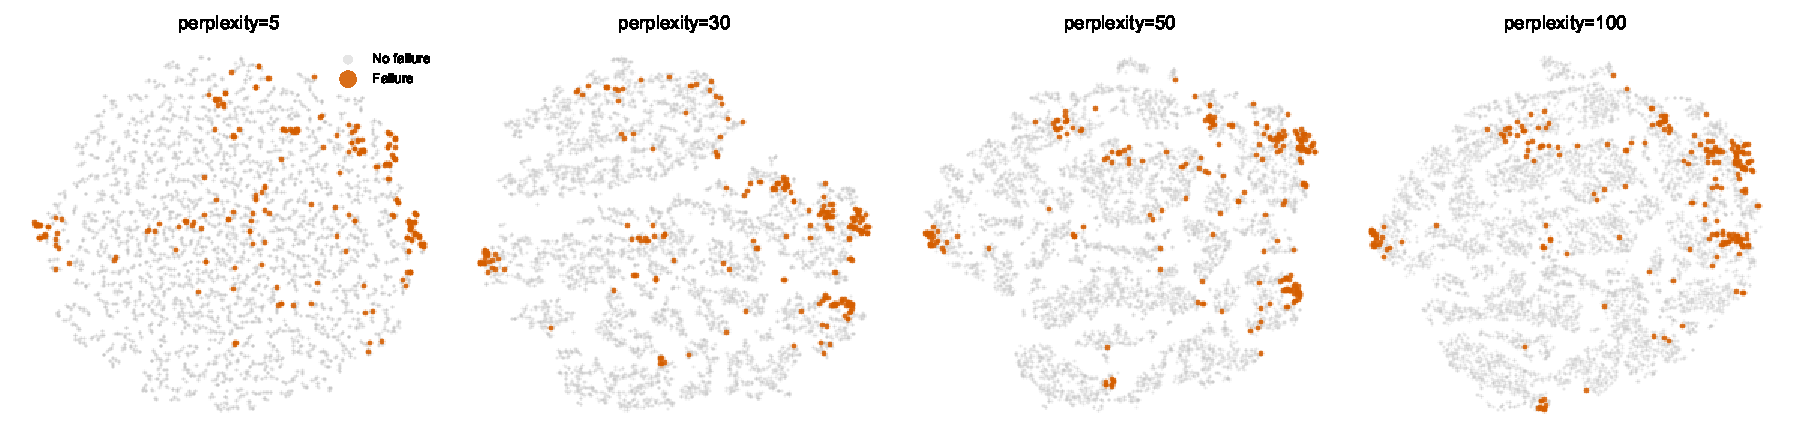
\includegraphics[width=0.9\textwidth]{tsne_perplexity.pdf}
\caption{t-SNE of the training data at perplexity 5, 30, 50, and 100. Failures (orange) occupy
consistent regions at every setting.}
\label{fig:tsne}
\end{figure*}

\begin{figure}[t]
\centering
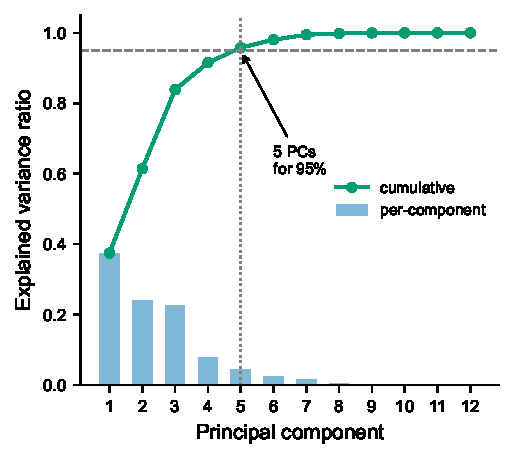
\includegraphics[width=0.72\columnwidth]{pca_elbow.pdf}
\caption{Explained variance of the principal components of the processed training features.}
\label{fig:elbow}
\end{figure}


\subsection{Predictive performance}
\label{sec:perf}

% Tree ensembles win; tuning trades recall for precision
\Cref{tab:models} lists positive-class test metrics. Tree ensembles outperform the linear and
instance-based models. Tuning raises F1 from 0.87 to 0.90, mainly through precision (0.86 to 1.00),
while recall falls from 0.88 to 0.82.

% Uncertainty is large with 34 failures
The test set contains 34 failures, so the uncertainty is large. The tuned model flags 28 rows, all of
them true failures: precision 1.00 (95\% CI 0.88--1.00), recall 0.82 (0.65--0.93), F1 0.90
(0.83--0.97), and ROC-AUC 0.984 (0.958--0.999). The scores are calibrated (Brier score 0.0095, against
0.033 for a constant prediction at the base rate; expected calibration error 0.007). Five-fold
cross-validation at the default threshold of 0.5 gives F1 $0.784 \pm 0.029$. \Cref{fig:pr,fig:cm}
show the PR curves and the confusion matrix.

% Prior work comparison, metric caveat
\Cref{tab:prior} compares these results with prior work. The studies differ in split and metric --
macro-F1 averages both classes, while positive-class F1 covers failures only -- so we report both
metrics where available.

\begin{table}[t]
\centering
\caption{Positive-class test metrics, sorted by F1.}
\label{tab:models}
\footnotesize
\begin{tabular}{@{}lrrrr@{}}
\toprule
Model & Prec. & Rec. & F1 & ROC-AUC \\
\midrule
XGBoost (tuned) & \textbf{1.00} & 0.82 & \textbf{0.90} & 0.984 \\
XGBoost & 0.86 & 0.88 & 0.87 & 0.988 \\
Random forest & 0.79 & 0.88 & 0.83 & \textbf{0.989} \\
Decision tree & 0.68 & 0.82 & 0.75 & 0.927 \\
MLP & 0.53 & \textbf{0.91} & 0.67 & 0.978 \\
SVM & 0.42 & 0.88 & 0.57 & 0.976 \\
$k$-NN & 0.43 & 0.79 & 0.56 & 0.877 \\
Logistic regression & 0.24 & 0.85 & 0.37 & 0.943 \\
\bottomrule
\end{tabular}
\end{table}

\begin{table}[t]
\centering
\caption{Comparison with prior results on AI4I~2020.}
\label{tab:prior}
\footnotesize
\begin{tabular}{@{}llr@{}}
\toprule
Study and protocol & Metric & Value \\
\midrule
Random forest, single split~\cite{physicsinformed2026} & pos.-class F1 & 0.722 \\
LightGBM, 5-fold CV~\cite{connectedvehicles2026} & macro-F1 & $0.814 \pm 0.012$ \\
Ours, single split & pos.-class F1 & 0.90 \\
Ours, single split & macro-F1 & 0.95 \\
Ours, 5-fold CV & pos.-class F1 & $0.784 \pm 0.029$ \\
\bottomrule
\end{tabular}
\end{table}

\begin{figure}[t]
\centering
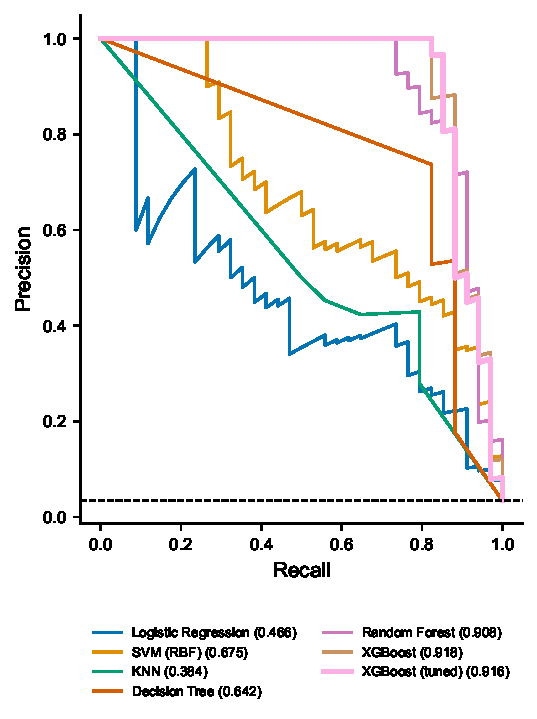
\includegraphics[width=0.7\columnwidth]{pr_curves.pdf}
\caption{Test PR curves; the tuned XGBoost model is highlighted. The dashed line is the 3.4\%
failure rate.}
\label{fig:pr}
\end{figure}

\begin{figure}[t]
\centering
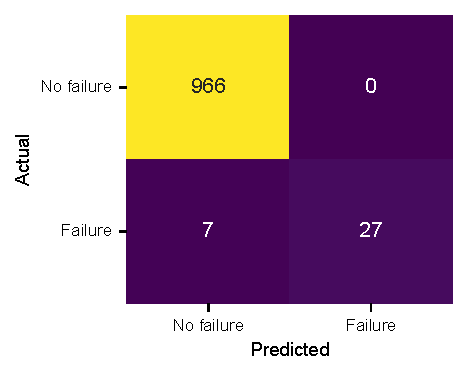
\includegraphics[width=0.6\columnwidth]{confusion_matrix_best.pdf}
\caption{Confusion matrix of the tuned model on the test set at the threshold selected on validation
data.}
\label{fig:cm}
\end{figure}

\subsection{Audit of the tuned model (H1)}
\label{sec:audit-results}


% H1 supported
The tuned model passes all four physical mechanisms (\cref{tab:audit}). On each mechanism's rows, its
relevant share exceeds that of all or nearly all permuted-label models; for PWF, $R = 0.686$ against a
permuted-model mean of 0.331. The highest-attribution feature on each mechanism's rows is one of its
trigger features. Restricting the audit to single-mechanism rows leaves every verdict unchanged and
raises each $R_m$, so rows with several mechanisms do not drive the result. RNF passes: the model is
not more concentrated on RNF rows than the permuted models are. Given the RNF label problem
(\cref{sec:setup}), we treat this check as weak. \Cref{fig:shap} shows the attribution matrix and the
global summary.

\begin{table}[t]
\centering
\caption{Audit of the tuned model. $R_m$: relevant share (RNF: share of the largest feature). Null:
mean over 100 permuted-label models. Single: rows with only mechanism $m$.}
\label{tab:audit}
\footnotesize
\setlength{\tabcolsep}{4pt}
\begin{tabular}{@{}lrlrrrr@{}}
\toprule
& $n$ & Top feature & $R_m$ & Null & $p$ & $p$ single \\
\midrule
TWF & 46 & tool wear & 0.309 & 0.143 & 0.020 & 0.010 \\
HDF & 115 & speed & 0.705 & 0.553 & 0.010 & 0.010 \\
PWF & 95 & power & 0.686 & 0.331 & 0.010 & 0.010 \\
OSF & 98 & overstrain ratio & 0.664 & 0.344 & 0.010 & 0.010 \\
RNF & 19 & speed & 0.168 & 0.218 & 0.970 & 0.891 \\
\bottomrule
\end{tabular}
\end{table}

\subsection{Controls and ablation (H2, H3)}
\label{sec:controls}

% Summary
\Cref{tab:controls} reports the audit for every variant.

% Permutation: H2 and H3
\textit{Permuted labels.} The model trained on permuted labels (test F1 0.08) fails all four physical
mechanisms, which supports H2. The naive null passes the same model on all four mechanisms
($p = 0.0005$ each), which supports H3.

% Shortcut: H2 with localization
\textit{Shortcut sensor.} With the weak shortcut, the model assigns little attribution to the sensor,
because the true HDF features determine HDF exactly, and the audit passes every mechanism. With the
strong shortcut, the sensor becomes the highest-attribution feature on HDF rows and $R_{\mathrm{HDF}}$
falls from 0.705 to 0.156, while TWF, PWF, and OSF still pass. The audit therefore identifies the one
affected mechanism. This model reaches test F1 0.86, higher than every non-XGBoost baseline in
\cref{tab:models}, so its accuracy gives no sign of the problem.

% Raw features: circularity addressed, HDF power limit
\textit{Raw features.} Without the derived features, test F1 falls from 0.90 to 0.84. TWF, PWF, and
OSF still pass ($p = 0.0099$), with raw trigger features ranked first (torque for PWF, tool wear for
OSF). HDF passes only at the threshold ($p = 0.0495$). Its trigger depends on the difference between
two temperatures, which trees approximate with many splits, and the permuted-label models already
place much attribution on the same three features (null mean 0.60). The audit has low power for a
mechanism defined by a difference of inputs unless that difference is a feature.

\begin{table}[t]
\centering
\caption{Audit $p$-values for each variant ($K = 100$; minimum 0.0099). Physical mechanisms pass if
$p < 0.05$ ($\times$ marks a failure); RNF passes if $p \ge 0.05$.}
\label{tab:controls}
\footnotesize
\setlength{\tabcolsep}{3pt}
\begin{tabular}{@{}lrrrrrr@{}}
\toprule
Variant & F1 & TWF & HDF & PWF & OSF & RNF \\
\midrule
Tuned model & 0.90 & 0.020 & 0.010 & 0.010 & 0.010 & 0.970 \\
\quad single rows & 0.90 & 0.010 & 0.010 & 0.010 & 0.010 & 0.891 \\
Raw features & 0.84 & 0.010 & 0.0495 & 0.010 & 0.010 & 0.376 \\
Weak shortcut & 0.86 & 0.010 & 0.010 & 0.010 & 0.010 & 0.822 \\
Strong shortcut & 0.86 & 0.010 & 1.00$\times$ & 0.010 & 0.010 & 0.366 \\
Permuted labels & 0.08 & 0.70$\times$ & 0.54$\times$ & 0.68$\times$ & 0.37$\times$ & 0.851 \\
\bottomrule
\end{tabular}
\end{table}

\subsection{Resampling and feature-space structure}
\label{sec:structure}




% Resampling result and its geometric effect
Borderline-SMOTE has the highest validation F1 among the oversamplers (\cref{tab:resamplers}).
\Cref{fig:boundary} shows the effect on a logistic regression fitted to a two-dimensional PCA
projection: without resampling, the decision boundary barely reaches the failure class, and each
oversampler moves it further into the majority class, trading precision for recall.

% Structure: nonlinear pockets consistent with separate mechanisms; robust to perplexity
\Cref{fig:dimred} projects the training data with PCA, t-distributed stochastic neighbor embedding
(t-SNE)~\cite{vandermaaten2008tsne}, and uniform manifold approximation and projection
(UMAP)~\cite{mcinnes2018umap}. In the PCA projection the classes overlap, which is consistent with
the low F1 of the linear models. In the nonlinear projections failures form several separate groups
rather than one region, which is consistent with several distinct mechanisms. Because t-SNE cluster
shapes depend on perplexity~\cite{wattenberg2016misread}, \cref{fig:tsne} repeats the projection at
four perplexities; the groups persist. \Cref{fig:elbow} shows that five of twelve principal
components are needed for 95\% of the variance, so the derived features are not redundant.

\begin{table}[t]
\centering
\caption{Oversampler comparison on the validation set (default XGBoost).}
\label{tab:resamplers}
\footnotesize
\begin{tabular}{@{}lrrrr@{}}
\toprule
Sampler & Prec. & Rec. & F1 & PR-AUC \\
\midrule
Borderline-SMOTE & \textbf{0.814} & 0.838 & \textbf{0.826} & 0.883 \\
SMOTE & 0.699 & \textbf{0.853} & 0.768 & \textbf{0.892} \\
ADASYN & 0.683 & 0.824 & 0.747 & 0.876 \\
\bottomrule
\end{tabular}
\end{table}


\subsection{Limitations}
\label{sec:limits}

% Synthetic ground truth
AI4I~2020 is simulated from the same rules we use as ground truth, so the ground truth is the
simulator's logic, not an independent measurement of real machines; we contribute a protocol, not a
finding about real equipment. Autran et al.~\cite{autran2024ai4ipmdi} show that realistic
irregularities added to AI4I~2020 change model performance, so results on the clean data may not
transfer.

% Audit-specific limits
The RNF check is weak, TWF has few rows and a partly random trigger, and with $K = 100$ several
$p$-values sit at the 0.0099 floor. The audit has low power for difference-based mechanisms, it
requires the trigger features $E_m$ to be known, and it needs mechanism labels for some failures. We
audit one model family with one explainer.

\section{Conclusion}
\label{sec:conclusion}

% Recap
We audited SHAP explanations of a PdM classifier against failure mechanisms that the model never
saw. Under a model-randomization null, the tuned model passes all four physical mechanisms, a model
trained on permuted labels fails all four, and a model with a shortcut sensor fails only the
mechanism the shortcut imitates. A naive null that compares random failure rows under the same model
passes the permuted-label model, so subgroup attribution tests need a null that accounts for how
atypical the audited rows are.

% Future work
The audit applies wherever maintenance records log a root cause for failures that a model predicts
as a binary risk; we have not measured how common such records are. Next steps are real maintenance
logs with recorded root causes, other explainers and model families, and a larger number of
permutations to resolve $p$-values below 0.01.

\section*{Acknowledgment}
Portions of the manuscript text and the analysis code were drafted with the assistance of an AI
system (Claude, Anthropic). The author reviewed and verified all content and takes full
responsibility for it. Code, model artifacts, and scripts that reproduce every number and figure are
available at \url{https://github.com/kowshik24/glowing-broccoli}.

\bibliographystyle{IEEEtran}
\bibliography{../refs}

\end{document}
